\documentclass[12pt,a4paper]{article}
\usepackage{graphics}
\usepackage{csvsimple}
\usepackage[russian,english]{babel}
\usepackage[utf8]{inputenc}
\usepackage[T2A]{fontenc} 
\usepackage{cmap}
\hoffset -1.6cm 
\textwidth  16.5cm 
\textheight 24cm 
%\topmargin -1cm 
\parskip 8pt 
\setlength{\unitlength}{1cm}
\sloppy
\addto\captionsenglish{
\renewcommand{\contentsname}{{\bf CO}ntents}
\renewcommand{\refname}{Bibliography}
\renewcommand{\figurename}{Figure}
\renewcommand{\tablename}{Table}
\renewcommand{\abstractname}{Abstract}
\renewcommand{\partname}{Section}
\renewcommand{\bottomfraction}{0.5}
\renewcommand{\floatpagefraction}{0.4}
\renewcommand{\textfloatsep}{0.5cm}
\renewcommand{\intextsep}{0.6cm}
\renewcommand{\floatsep}{0.3cm}
}

\begin{document}
%..................................................................
\begin{titlepage}
\par 
\vspace*{-2cm}
\begin{center}
{\sf \Large
\vspace*{1.5cm}
{\Huge Семенов, 8-й семестр, 2017}\\
{ Все, что вы хотели {\small(или не хотели, но сдавать надо)} знать о философии,\\ но боялись спросить}}\\
\vspace*{2cm}
\scalebox{1.2}{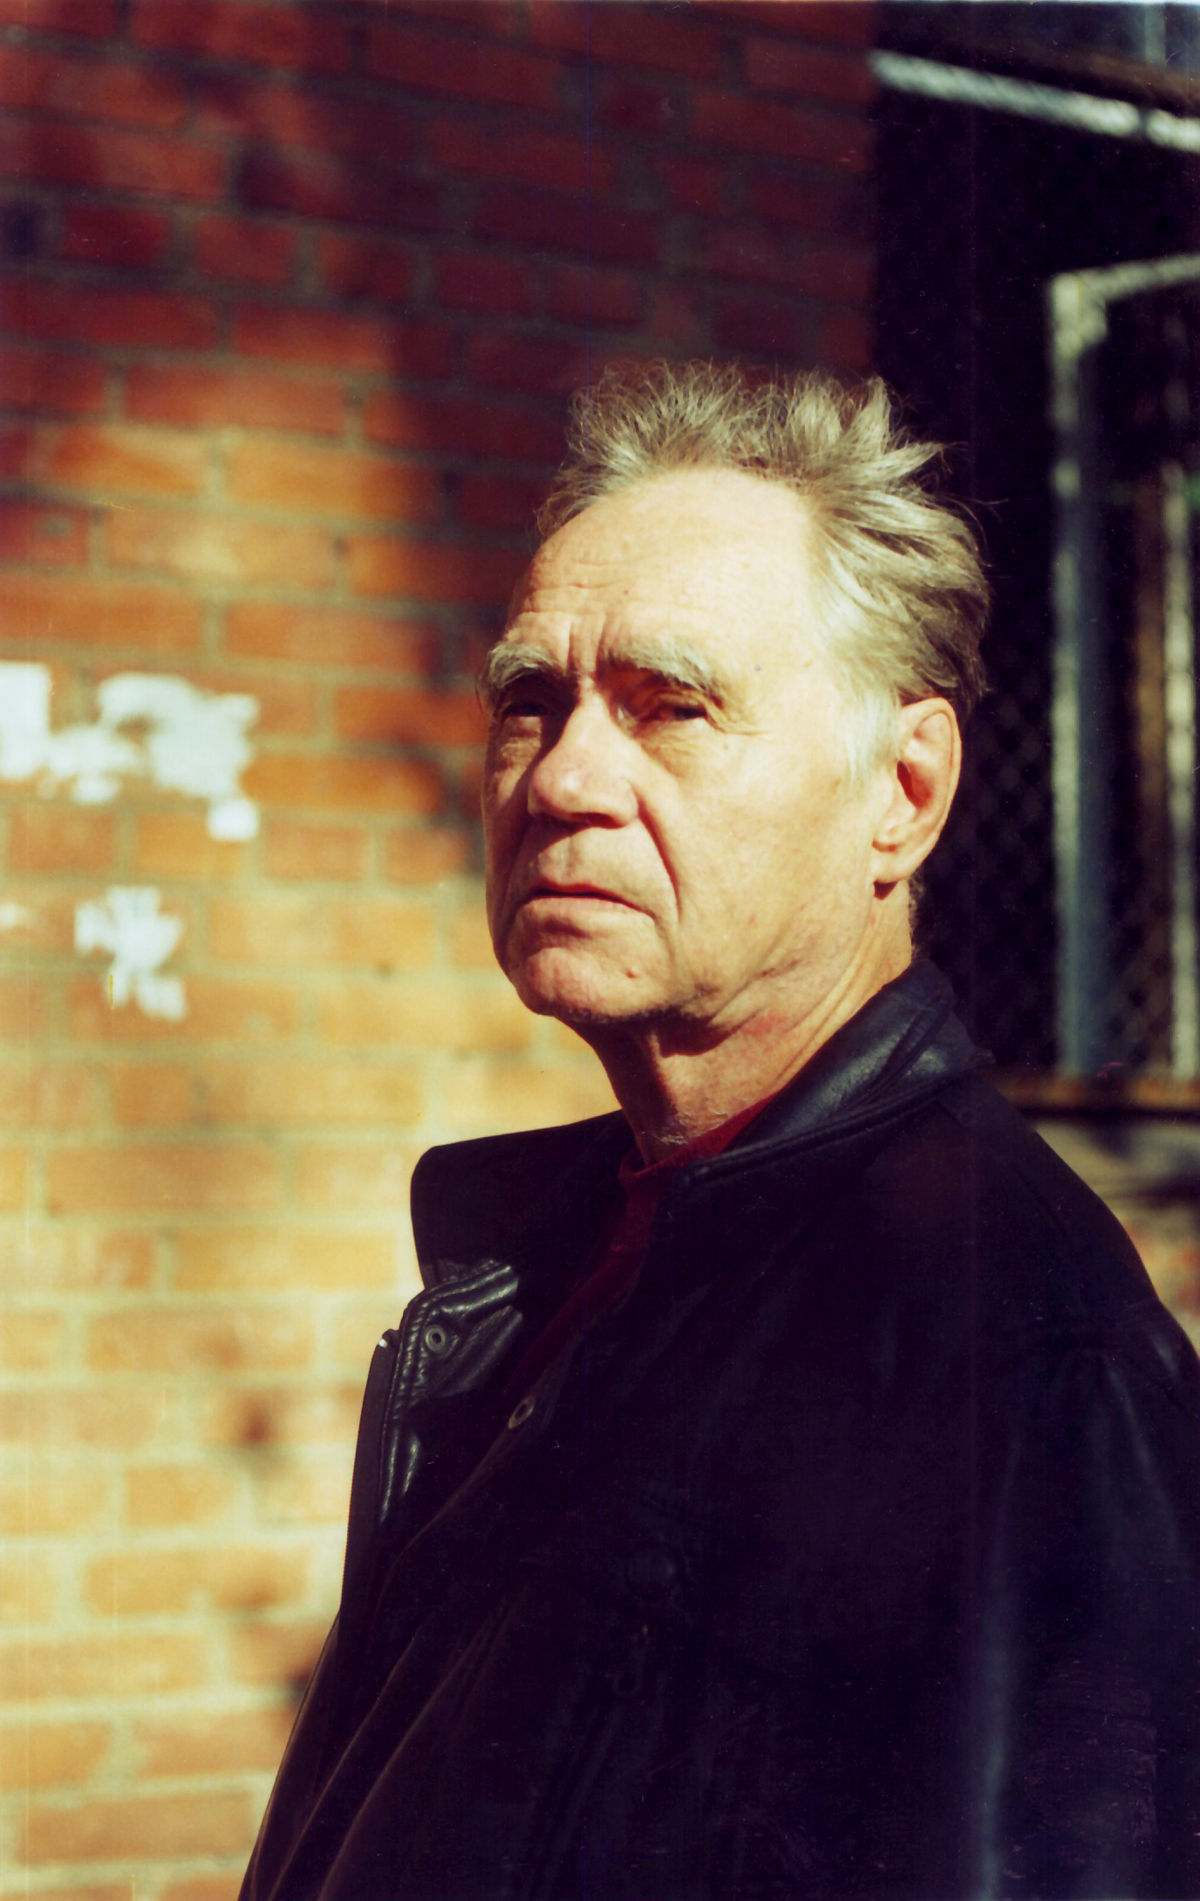
\includegraphics{thegod.png}} 
\begin{flushright}
\sl\small
by Nyaxx11k aka KingKO,\\
Institute for Porn and Pederasts,\\
Chair of Roosterology
\end{flushright}
\end{center}
\end{titlepage}
%..................................................................
\topmargin -1cm 
\hoffset -0.7in 
\textwidth 6.0in 
\textheight 9.0in 
\normalsize 
\pagenumbering{arabic}
%----------------
\tableofcontents
\pagebreak
%----------------

\section{Истина как цель научного исследования. Истина и заблуждение.}
Согласно т.н. "Классическому определению истины", \textbf{истина} - это то, что согласуется с действительностью. 
Соответственно \textbf{заблуждение} - то, что с действительностью не согласуется. \textit{Не ложь - это отрицание истины исключительно в матлогике. В остальных науках это - умышленное введение в заблуждение.}
Ясно, что все науки занимаются поиском истины.
Каждая из них ищет истину о чем-то своем: биология - о живых организмах, физика - о предельно общих законах природы и т.д.

\section{Истина как объект философского исследования.}
Ясно, что все науки занимаются поиском истины.
Каждая из них ищет истину о чем-то своем: биология - о живых организмах, физика - о предельно общих законах природы и т.д.
\textbf{Философия} же ищет истину о самой истине: как достичь истины, не свалившись в заблуждение.

\section{Философия как теория познания и самый общий метод мышления.}
Философия ищет истину о самой истине: как достичь истины, не свалившись в заблуждение.
То есть философия является теорией познания (\textbf{гносеологией}/\textbf{эпистемологией}).
По другому задача философии может быть сформулирована так: как мыслить правильно, т.е. так, чтобы прийти именно к истине.
А это означает, что философия дает наиболее общий метод мышления. 

\section{Понятие объекта и субъекта, объективного и субъективного}
\textbf{Субъект} - это существо, обладающее сознанием и волей, и способное к целенаправленной деятельности,
которую оно направляет на \textbf{объект} - некий предмет/явление.
У нас в курсе деятельность - это познание.
Т.е. субъект познает объект.
\textit{Да, субъект может быть и объектом. Семенов грозился просить привести примеры объектов.
Да, называем все, что видим, и будет счастье.} 
Соответственно, вводят понятия \textbf{субъективного} - оно означает, что что-то зависит от субъекта,
и \textbf{объективного} - того, что от субъекта не зависит.

\section{Ступени человеческого познания}
У человека есть два способа познания - \textbf{чувственное познание} и \textbf{мышление} (ака \textbf{умственное познание}).
Первое осуществляется органами чувств и человеку неподвластно.
А второе - это человеческая деятельность, она подвластна сознанию, а значит, и методологию для нее можно разрабатывать (более того, это-то и есть философия как метод мышления).

\section{Чувственное познание. Его основные формы.}
Чувственное познание существует в трех формах, или, скорее, стадиях:
\begin{enumerate}
\item \textbf{Ощущение} - начальная фаза. Объект воздействует на субъекта, и его органы чувств (всего их 5) передают информацию об этом в мозг.
\item \textbf{Восприятие} - на этой ступени данные со всех органов собираются в единый образ предмета.
\item \textbf{Представление} - образ ранее воспринятого предмета может быть воспроизведен в сознании субъекта и в отсутствии этого предмета.
\end{enumerate}
Это познание есть не только у человека, но и у любых животных. Понятно, что чувственного познания не достаточно для того, чтобы познать закономерности мира.

\section{Мышление как деятельность человека. Проблема правильного образа (метода) познания. Философия как метод мышления и наука о мышлении - логика}
\textbf{Мышление} - это уже человеческая деятельность, она подвластна сознанию, а значит, и методологию для нее можно разрабатывать, в отличие от чувственного.
Более того, этим-то и занимается философия.
Значит, философия является еще и наукой о мышлении - логикой.
\textit{Вообще, \textbf{логика} - это наука
о мышлении, в центре внимания которой - его правильность или истинность.\nocite{Sem01} Далее мы увидим, что не все - философия, что логика.
}
\textit{ Следует оговориться, что его она изучает как способ достижения истины, т.е. не интересуется, например, отклонениями в мышлении (это к психиатрам)}
\textit{ При мышлении органы чувств не используются непосредственно. }

\section{Два вида мышления: рассудочное и разумное, и две логики: формальная и содержательная (философская)}
Мышление может быть как субъективной деятельностью - \textbf{рассудочным мышлением},
так и объективным процессом - \textbf{разумным мышлением}. 
У каждого из них логика своя - соответственно, \textbf{формальная} и \textbf{содержательная}.
Формальная логика изучает лишь правильность мышления, а посему от философии с проблемами истины она давно отпочковалась, став самостоятельной наукой. Логика же разумного мышления в философии используется интенсивно. 
\textit{ Это не значит, что философия забивает на чувственное познание и рассудок, и уж тем более, что она их отрицает. Очевидно, для работы разума нужны как чувственные данные, так и рассудок - чтобы стать известными, результаты работы разума в любом случае нужно перевести в формы, присущие рассудку.}

\section{Классическое определение истины}
Без лишних предисловий: \textbf{Истина} - это то, что согласуется с действительностью (\textit{by Платон/Аристотель-у первого оно встречается раньше, но приписывают обычно второму}). 
Т.е. иначе говоря, истина - соответствие между миром и сознанием.

\section{Проблема определения понятий "мир" и "сознание"}
Обычно дают определение через род и видовое отличие. Мир и сознание - предельно общие понятия, еще более общее только одно - бытие (т.е. и мир, и сознание - есть): но это нам ничего не даст - бытие и так все включает. Значит, придется раскрывать отношение - что из них первично, что вторично. Это - \textbf{"основной вопрос философии"}. Именно по ответу на него классифицируют направления философии.

\section{Основной вопрос философии}
Обычно дают определение через род и видовое отличие. Мир и сознание - предельно общие понятия, еще более общее только одно - бытие (т.е. и мир, и сознание - есть): но это нам ничего не даст - бытие и так все включает. Значит, придется раскрывать отношение - что из них первично, что вторично. Это - \textbf{"основной вопрос философии"}. Именно по ответу на него классифицируют направления философии. \textit{Кстати, философ, считающий, что нет никакого основного вопроса - недофилософ и петух. Считающий, что на вопрос нет и не будет ответа - это уже другое.}

\section{Философия как мировоззрение (онтология). Натурфилософия. Социальная философия.}
Итак, определить мир и сознание можно только одним образом - раскрыв отношение между ними. Это значит, что тем самым будут определены оба понятия. Тем самым философия дает еще и предельно общий взгляд на мир, т.е. является \textbf{онтологией}. Раньше, когда науки еще были в зачаточном состоянии, только философия была готова дать хоть какую-нибудь картину мира. Такое учение называется \textbf{натурфилософией}. В настоящее время натурфилософия отмерла за ненадобностью. \textit{Но не онтология - она по прежнему занимается проблемами мира - теми, которые нужны для теории познания}. Но кроме природы есть еще общество - им занимаются \textbf{социальная философия} и \textbf{философия истории}. И с ними все не так однозначно, как с натурфилософией. Во-первых, есть \textbf{общественное сознание} - в широком смысле это все знание человечества; более того, сознание отдельного человека формируется в обществе \textit{(а дети-Маугли ни говорить, ни социализироваться не могут)}. Во-вторых, разные школы придерживаются разных взглядов на общество: первые говорят, что общество - только название, а на самом деле есть только взаимодействующие люди. Вторые таки признают общество. Это два направления - \textbf{социальный номинализм} и \textbf{социальный реализм} соответственно.

\section{Материализм как онтология и как гносеология. Понятие материи.}
Итак, первое направление в философии \textit{(кстати, именно его и придерживается Семенов)} - это \textbf{материализм}: первичен мир, сознание вторично. Т.о. материализм признает объективную реальность - \textbf{материю}.

\section{В чем заключается вторичность сознания по отношению к материи.}
Нельзя сказать, что материалисты объявляют, что сознания нет вообще. Просто сознание не образует отдельного мира, оно зависимо от материи и не существует без нее. Действительно, сознание - продукт мозга, который есть ни что иное, как материя. Но это не самое главное. А самое главное в том, что сознание - \textsl{отражение} материи.

\section{Формы материализма. Натурматериализм и панматериализм.}
Материалисты до Маркса были непоследовательны: в природе они были материалисты (\textbf{натурматериалисты}) при переходе к обществу им приходилось переходить на позиции идеализма. Действительно, казалось бы, общество - это отражение сознания людей. 
\textit{Еще бы, общество в отличие от физических тел не пощупаешь.}
\textit{Не говоря уже о том, что общество в отличие от мира не вечно - оно возникло вместе с людьми.} Маркс же нашел социальную материю - производственные отношения. Тем самым материализм стал полным -\textbf{панматериализмом}, или \textbf{диалектическим материализмом}. Другое важное его следствие - человек не просто пассивный наблюдатель, он воздействует на мир, преобразуя его.

\section{Субъективный идеализм. Солипсизм. Трудности субъективного идеализма.}
Итак, идеализм дает прямо противоположный материализму ответ: сознание первично, мир вторичен.  Первый его сорт - \textbf{субъективный идеализм}: мир существует только в моем сознании. Представитель такого течения - Беркли (правда, на старости лет он ушел в объективные идеалисты).\textit{Тут так же, как и с материалистами: мир не отрицается, а существует как комплекс моих восприятий}. Люди тоже существуют в моем сознании как духи.
Точка зрения, когда мир есть лишь форма существования моего сознания, называется \textbf{солипсизмом}. Т.е. все, что не воспринимается, не существует. Что происходит с миром, когда я его не ощущаю (сплю, например)? Беркли вкрутился тем, что ввел других мыслящих духов, которые воспринимают мир в мое отсутствие (\textit{"Стоп, люди же тоже должны пропадать, когда я сплю... А, неважно"}) А как мои представления отличать от восприятия? Очевидно, что воображаемым яблоком наесться нельзя. Вот тут и приходится вводить абсолютный дух, который бы отделял представление от восприятия. А это уже попахипает \textbf{объективным идеализмом}. Точнее, им и является. \textit{Другие пытаются отгородится софизмами.} Но субъективный идеализм - не просто глупость. Это, скорее, раздувание до неприличия одного из моментов отношения сознания и объективного мира.

\section{Объективный идеализм. Суть и основные компоненты.}
Итак, идеализм дает прямо противоположный материализму ответ: сознание первично, мир вторичен. Его второй сорт - \textbf{объективный (абсолютный) идеализм}. Его фундамент заложен еще пифагорейцами и Платоном, из тех, кто поновее - Шеллинг и Гегель. Чтобы избавиться от багов солипсизма, вводят \textbf{абсолютный дух}, который бы отделял представление от восприятия. Этот дух - вне человека и человечества. Он творит (мыслит) природу. А духи людей уже отражают эту природу. Итого насчитываются три источника и три составные части объективного идеализма:
\begin{enumerate}
\item Абсолютный дух
\item Природа
\item Остальные духи (люди тут).
\end{enumerate}
\textit{Абсолютный дух кажется похожим на Бога, но мешать идеалистов и верунов нельзя - Семенов опустит тут же! И поделом: философия и религия - две большие разницы. Здесь и далее, вплоть до христианской философии, слово "Бог" означает скорее "абсолютный дух", чем "бородатый дяденька на небе, запиливший этот мир за семь дней (или за шесть?)"}

\section{Социоконструктивный идеализм}
Его основоположник и ярчайший представитель - Фихте. Центральное понятие у него - Я. \textit{Еще один субъективный идеалистишка? Как бы не так!} Этот Я - общественный разум, творящий мир. Это не Я индивидов, и даже не их прямая сумма. Это - объективный дух по отношению к людям. Но в отличие от объективных идеалистов, Я не существует без индивидов. Это абсолютное Я творит не-Я.

\section{Монизм. Два его вида: материализм и идеализм}
Нам потребуются понятия \textbf{субстанции} и противоположного ему \textbf{акциденции}. 
\textbf{Субстанция} - это бытие, существование которого не обусловлено никаким другим бытием,
находящимся за его пределами.
А \textbf{акциденция} - это бытие производное, имеющее началом
что-то отличное от него самого. Теперь философские течения можно классифицировать по числу субстанций. Материализм и идеализм - \textbf{монизмы}, т.е. у них только одна субстанция (материя или дух соответственно). \textit{Есть еще монисты - маргиналы, у которых субстанцией является не мир и не сознание, а что-то еще: ощущения/жизнь/экзистенция. Вроде этих петушков можно свести к идеалистам, если вычистить словоблудие, прикрываемое терминами.}

\section{Понятие субстанции и акциденции}
\textbf{Субстанция} - это бытие, существование которого не обусловлено никаким другим бытием,
находящимся за его пределами.\\
\textbf{Акциденция} - это бытие производное, имеющее началом
что-то отличное от него самого.

\section{Дуализм и плюрализм}
Напомню, \textbf{субстанция} - это бытие, существование которого не обусловлено никаким другим бытием,
находящимся за его пределами,
а \textbf{акциденция} - это бытие производное, имеющее началом
что-то отличное от него самого. \textbf{Дуализм} - это философское течение с двумя субстанциями. Его сторонником был, к примеру, Декарт. У него мир (протяженная субстанция) отдельно, сознание (мыслящая субстанция) отдельно. Но мыслящую субстанцию он делил на Бога и человеческую душу. А Бог создал все, в том числе и протяженную субстанцию, а потом просто забил на нее. Т.е. она и не очень-то и субстанция. Таким образом, Декарт не стоял целиком на позициях дуализма, а был эклектиком - с уклоном в объективный идеализм. 

А \textbf{плюрализма} - течения с более чем двумя субстанциями, придерживался Лейбниц. Правда, у него градус эклектики был не ниже - вводя субстанции - монады, которые вечны, он вводит также и Бога, который их все же может уничтожать и создавать. 


\section{Агностицизм (феноменализм)}
Наконец, есть течение, в котором субстанций - неопределенное количество. Т.е. человечество не знает ответа на основной вопрос, и не узнает никогда. Это - \textbf{агностицизм} ака \textbf{феноменализм}, и его создатель - Юм \textit{(вообще-то он Хьюм - Hume)}. Согласно Юму, чувственные данные - единственное, что мы знаем о мире. Чтобы ответить на основной вопрос, нам нужно выйти за рамки наших чувств. \textit{Не путать со скептиками-они не отрицают познаваемость, а только сомневаются}.


\section{Позитивизм: первый, второй и третий. Постпозитивизм. Аналитическая философия.}
\textit{Черти, причем очень популярные - Бертран Рассел, Карл Впоппер - это все сюда. Семенов говорит, что это наиболее популярная философия, по крайней мере, на Западе.}
\begin{enumerate}

\item 1-я волна. Конт, Милль, Спенсер.
\textit{Хотели очистить философию от метафизики. В результате - дикая эклектика.} Едиственный источник знания - эмпирический.
\item 2-я волна ака \textbf{эмпириокритицизм}. Авенариус, Мах.
Мешанина из субъективного идеализма и агностицизма. Вводят "элементы мира", и объявляют, что все вещи из них состоят. В результате эти элементы оказались ощущениями.
\item 3-я волна ака \textbf{неопозитивизм}. Родился из \textbf{аналитической философии} (Мур, Рассел, Витгенштейн), которая основной целью ставила  анализ языка (ибо чувственные данные именно в языковую форму и пакуются). Представители - Карнап, Франк, Гедель, Шлик. Это также известно как \textbf{логический позитивизм}, некоторые даже отделяют его от аналитической философии. \textit{Рухнул с позором}.
\item \textbf{Постпозитивизм} (Поппер, Кун, Лакатос, Фейерабенд).
\textit{Я просто оставлю это здесь:\\
"...Возникший в результате кризиса неопозитивизма новый вариант позитивизма —
постпозитивизм в лице, если не всех, то по крайней мере ряда его крупнейших
представителей, встал на путь прямой дискредитации науки. Тенденции, отчетливо
наметившиеся в работах Т. Куна (1922-1996), нашли свое завершение в сочинениях
П. Фейерабенда (1924-1994). Согласно утверждениям последнего, теории науки
имеют нисколько не больше ценности, чем мифы, сказки, религиозные учения. А
раз так, то наука ни в коей мере не может быть использована для опровержения
феноменализма. Так, философское направление, объявлявшее себя ни мало ни
много, а философией науки, превратилось в конце концов в теоретическое
обоснование и оправдание любых лженаучных построений и вообще любого
мракобесия, включая религиозное..."\\
Короче, позитивизм - курятник.
}
\end{enumerate}

\section{Основные эпохи истории человечества.}
\begin{enumerate}
\item Зарождение человека - 1.9 млн лет назад
\item Современный человек появился 40 тыс. лет назад.
Тогда было только житейское знание и \textbf{первобытный коммунизм} - общество было бесклассовым.
\item Потом появилась цивилизация  - уже с \textbf{классами}. Ее основные признаки - монументальные сооружения и письменность.
31 век д.н.э-9 век д.н.э - \textbf{эпоха Древнего Востока}. Представлена в основном Древним Египтом и Шумерами (потом уже появились Индская цивилизация, Шань и гипотетическая Ся).
Там возникла преднаука - знание уже собиралось и фиксировалось, но анализа причин и доказательств не было.
Строй там был интересный - Маркс назвал его "\textbf{азиатский}", Семенов же называет его \textbf{политарным}. Некоторые историки говорили, что там был рабовладельческий строй, но это неверно - рабы там не играли роли.
\item 8 в.д.н.э-5 в.н.э. - \textbf{Античная эпоха}. Там появилась наука, философия, и там было \textbf{рабство}.
\item 6 в.н.э-15 в.н.э. - \textbf{Средневековье}. Там \textbf{феодализм}.
\item 16 в.н.э-1914/1917 - \textbf{Новое Время}. Там \textbf{капитализм}.
\item 1914/1917-наше время - \textbf{Новейшее время}. Там все еще пока \textbf{капитализм}.
\end{enumerate}
\textit{Напомню - \textbf{частная собственность}-это собственность, позволяющая одним людям эксплуатировать других. С \textbf{личной собственностью} ее путать нельзя.}

\section{Возникновение классового общества. Эпоха Древнего Востока. Общественный строй Древнего Востока. Появление письменности и преднауки.}
\textbf{эпоха Древнего Востока} была в 31 век д.н.э-9 век д.н.э. В нее появилась \textbf{цивилизация}-классовое общество, города, монументальные сооружения и письменность (пока - в виде иероглифов на камне/папирусе). Тем самым знание стало фиксироваться. Это еще не наука, потому что анализа знанй, поиска причинно-следственных связей и доказательств не было - только готовые рецепты (\textit{"А вывести формулу можете? Нет? На пересдачу!"}). Знание было общим - содержало и астрономию, и медицину, и математику. Маркс назвал его "\textbf{азиатский}", Семенов же называет его \textbf{политарным}. При нем есть работники и управляющие. Средства производства принадлежат управляющим, но не каждому по отдельности а все всем сразу. \textit{Поэтому-то в СССР и говорили, что в эту эпоху было рабство. Уж больно похожи госпредприятия и номенклатура на Древний Египет. Семенов характеризует строй СССР как \textbf{индустриальный политарный}.}

\section{Античное общество и античная эпоха. Возникновение в античном мире теоретического мышления, философии и науки.}
Говоря об античной эпохе (8 в.д.н.э-5 в.н.э.), нужно первым делом упомянуть Древнюю Грецию. Это было не цельное государство, а скорее сеть из ~260 полисов, разбросанных по Греции, Италии, побережью Средиземного Моря и его островам. Т.е. от северной Африки до южной Франции и побережья Черного моря. Там было \textbf{рабство} - захваченные на войне люди лишались всех прав и отправлялись на работы. За 6-7 лет человек изнашивался и умирал.  Политические режимы в Греции были разнообразными - от \textbf{тирании} до \textbf{демократии}. Именно в Древней Греции появились науки, в т.ч. философия, и теоретическое мышление.

Второе важное государство - это Древний Рим. Рим возник еще в 8-м веке д.н.э., однако влияние он стал набирать только в 3 в. д.н.э., уже после развала империи Александра Македонского. Тогда Рим был республикой. Потом, уже в 1-м веке д.н.э., появилась Римская Империя. Ее развал (или, скорее, раскол на Западную и Восточную) империи в 476 году н.э. считается концом античности.

\section{Милетская школа. Проблема, которую она стремилась решить.}
\ \ \ \
\underline{Фалес ($\approx$624 д.н.э - $\approx$546 д.н.э.)}. Город: Милет, Малая Азия.

Математик, астроном, философ. Первый доказал теорему (\textit{да-да, ту самую, про параллельные прямые и угол}). Предсказывал затмения. В плане философии же - основатель \textbf{Милетской школы}, да и вообще \textbf{философии}. Считал, что в мире есть первовещество, и все сущее - его проявления. Фалес считал это первовещество \textbf{водой} (\textit{скорее, это нечто абстрактное, текучее и жидкое, а не буквально вода из моря}). А так как все движется и меняется, то есть и движущая сила - \textbf{душа, "психе"}.

\underline{Анаксимандр ($\approx$619 д.н.э - $\approx$546 д.н.э.)}. Город: Милет, Малая Азия.

Создатель первых солнечных часов, первой карты.
Считал, что в мире все движется по единым законам. Человек у него - потомок морских животных, а мир имеет вид вращающегося цилиндра. Его осколки улетели и образовали звезды и Солнце с Луной. Причем таких цилиндров бесчисленное множество, мы - на одном из них.
По его мнению, в мире есть первопричина, первовещество. В отличие от Фалеса, считал им нечто неопределенное -т.н. \textbf{апейрон}. Он неосязаем и доступен только уму.

\underline{Анаксимен ($\approx$585 д.н.э - $\approx$525 д.н.э.)}. Город: Милет, Малая Азия.

У него мир имеет вид неподвижного диска. 
Первовеществом у него был \textbf{воздух}, превращающийся во все остальное в результате разрежения и сгущения.

Главный же вопрос - мир вечен, но в нем нет ничего вечного. Что же делает мир вечным? Именно это и было причиной введения первовещества. Сходные взгляды высказывал \underline{Гераклит}. Его и милетцев иногда даже объединяют в \textbf{Ионийскую школу}.

\section{Гераклит Эфесский.}
\ \ \ \
\underline{Гераклит ($\approx$540 д.н.э - $\approx$480 д.н.э.)}. Город: Милет, Малая Азия.

Как и милетцы, считал мир вечным, в котором нет ничего вечного. Тоже вводил первовещество - на этот раз \textbf{огонь}: "Мир был, есть и будет огнем, вечно разгорающимся и утихающим". Но интересен он также тем, что видел движущую силу в противоречивости этого мира (\textit{по типу "нож-это оружие, но в руках хирурга он спасает жизни и т.д."}). Получается, мир состоит не из набора вещей, а из процессов. Т.о. Гераклит - создатель \textbf{диалектики}. 

\section{Пифагор и пифагорейцы.}
\ \ \ \
\underline{Пифагор ($\approx$570 д.н.э - $\approx$487 д.н.э.)}. Родился на острове Самосе, но жил и работал в южной Италии.

Сторонник аристократии, поэтому свалил сначала с Самоса с его тираном, а потом из Кротона после демократического переворота.
Основатель пифагорейской школы. Доказал теорему имени себя.

Выделял три области исследований - религию, этику и науку. Пифагор и пифагорейцы чуть ли не обожествляли числа: все явления - это числа. Мир описывали как центральный огонь (\textit{не Солнце}), вокруг которого вращаются десять сфер: пять планет, Земля, Солнце, Луна, Млечный путь и Антиземля (чтобы всего было десять). Делили все на десять пар противоположных понятий, например: "четное-нечетное", " мужское-женское", "четырехугольное-многостороннее","свет-тьма" и т.д.

\section{Элейская школа. Основные ее представители. Учение Парменида о бытии. Вклад элеатов в развитие философской мысли.}
\ \ \ \
\underline{Ксенофан ($\approx$580 д.н.э - $\approx$490 д.н.э.)}. Бродячий певец родом из Малой Азии, обошел всю Грецию. \textbf{Пантеист}-отождествлял Бога и природу, бытие. Мифологию Древней Греции не признавал, считал выдумкой людей.

\underline{Парменид ($\approx$546 д.н.э - $\approx$470 д.н.э.)}. Город Элея, это в Италии.

\scalebox{0.38}{
\includegraphics{COmic-parmenides.jpg}}

Что такое бытие? Это - то, что есть. А небытие? То, чего нет. Раз так, то бытие вечно, иначе откуда оно пришло и куда уйдет? В небытие? Так некуда, получается. А раз так, то и в мире ничто не появляется и не исчезает и не меняется. Итого есть только неподвижное и единое (иначе два бытия отграничены небытием) бытие, а наши чувства нас обманывают. А это, кстати, уже важная мысль - Парменид поделил познание на чувственное и умственное. 

\underline{Зенон Элейский \textit{(не путать с Китийским-тот был стоик!)} ($\approx$490 д.н.э - $\approx$430 д.н.э.)}. Ученик Парменида, доказывал своего учителя \textbf{апориями} - парадоксами, из которых следовала невозможность движения. До нас дошло не все. Например: "Летящая стрела неподвижна, так как в каждый момент времени она занимает равное себе положение, то есть покоится; поскольку она покоится в каждый момент времени, то она покоится во все моменты времени, то есть не существует момента времени, в котором стрела совершает движение." Или про Ахиллеса, черепаху и сходимость рядов.

\underline{Мелисс ($\approx$485 д.н.э - $\approx$425 д.н.э.)}. Его важнейшее положение - бесконечность мира не только во времени, но и в пространстве. Опять же, явления - видимости, а есть только сущности.

\textit{И напоследок еще раз следует подчеркнуть: раз чувства нас обманывают, какое-то движение подсовывают, то истину необходимо постигать \textbf{разумом}.}

\section{Эмпедокл и Анаксагор.}
\ \ \ \
\underline{Эмпедокл ($\approx$492 д.н.э - $\approx$430 д.н.э.)}. Жил на острове Сицилия.

Вводил четыре элемента: огонь, воду, землю и воздух. Они вечны, а все сущее - результат смешения этих стихий под действием двух сил - \textbf{дружбы и вражды}. \textbf{Редукционист} - сводит вещи к смеси старых качеств. История у него разбита на 4 фазы:
\begin{enumerate}
\item Вначале была дружба
\item Потом появилась вражда, но влияние дружбы еще решающее
\item Потом только вражда
\item И наконец, происходит переход от вражды к дружбе. Мы именно в эту эпоху и живем.
\end{enumerate}
У него было много интересных мыслей - про конечность скорости света, про естественный отбор (правда, это было скорее соединение нежизнеспособных органов в монстров, которые в итоге стали гармоничными и способными к размножению). А ощущение он понимал так: частицы стихий стряхиваются и попадают на наши органы чувств.

\underline{Анаксагор ($\approx$496 д.н.э - $\approx$428 д.н.э.)}. Родился в Клазоменах, Малая Азия. Переехал в Афины, был другом Перикла, который даже спас его от кары за безбожие.

У него есть семена мира, их, в отличие от Эмпедокла, бесчисленное множество. Движущая сила, объединяющая их - \textbf{ум (нус)}. Т.е. тела - просто смешение семян мира.

\textit{Но это еще не атомизм. И у одного, и у второго, стихии были бесконечно делимы.} 

\section{Древнегреческий атомизм. Возникновение абсолютного детерминизма.}
\ \ \ \
\underline{Демокрит ($\approx$460 д.н.э - $\approx$360 д.н.э.)}. Город: Абдеры, во Фракии.

Ярчайший представитель \textbf{атомистического материализма}.
Ученик Левкиппа, который и предполагается как создатель сего направления \textit{(но увы и ах, данные неточные)}.
Его взгляды неясны до конца - возможно, его точка зрения менялась в процессе. Основные же положения:
есть пустота, небытие. В ней есть мельчайшие неделимые частицы - \textbf{атомы}\textit{(Неделимые? Резерфорд, Кюри и Майтнер под столом.)}. Эти атомы обладают весом, формой и незримы. Из них-то все и состоит. Да, и чувства нас опять-таки обманывают. Мир не такой, как в сознании. \textit{Говорят, на старости лет даже глаза себе выколол, чтоб постигать мир исключительно разумом}. И важнейшее его открытие - \textbf{детерминизм}. Атомы подчиняются всеобщим законам, а значит, все имеет причину и предопределено. Необходимость тоже всеобщая. \underline{Эпикур} впоследствии взял атомизм на вооружение, но детерминизм отвергал - у него была случайность и свобода воли.

\section{Софисты. Протагор и Горгий.}
Софисты были в 6-5 вв д.н.э. Они были профессиональными ораторами. Обучали риторике и философии, ибо умение отстоять свою точку зрения было необходимо (демократия-выборы, суды без прокуроров/адвокатов). Умели доказать что угодно.
\textit{\\-Это собака - твоя?\\ -Ну да, я ее хозяин.\\-А она часом не мать?\\-Ну мать, вон у нее щенки бегают.\\-Ага, значит она твоя и мать. Значит, ты - сукин сын. q.e.d.}
Подразделяются они на старших и младших. Протагор и Горгий - оба старшие.

\underline{Протагор ($\approx$486 д.н.э - $\approx$411 д.н.э.)}. Город: Абдеры, во Фракии.

Считал, что человек - мера всех вещей. А раз так, то и у каждого своя правда. Истина есть то, что приносит пользу. А полезность субъективна.

\underline{Горгий ($\approx$480 д.н.э - $\approx$380 д.н.э.)}. На протяжении жизни жил в Италии, Афинах, умер в Ларисе. 

Горгий in a nutshell:
\begin{enumerate}
\item Ничто не существует.
\item Если же и существует, то не познаваемо.
\item Ну а если и познаваемо, то языком непередаваемо.
\end{enumerate}

\textit{Короче, в этих учениях образ жизни софистов виден насквозь}.

\section{Сократ.}
\ \ \ \
\underline{Сократ ($\approx$469 д.н.э - $\approx$399 д.н.э.)}. Афинянин.

 Книг не писал, вел беседы (называл методику \textbf{майевтикой} - искусством повивальной бабки): вначале включал иронию, и когда оппонент понимал, насколько безблагодатная у него точка зрения, Сократ наводящими вопросами помогал ему родить мысль. Был обвинен в развращении молодежи и богохульстве. Приговорен к казни и выпил яду.

Что же касается его философских воззрений, то он считал, что добродетель проистекает из знания: "никто не желает зла по своей воле - зло от незнания". Спорами восстанавливал авторитет истины, опущенной софистами. 
Тремя главными добродетелями считал мужество, справедливость и умеренность. Говорил, что круг потребностей нужно ограничить, чтобы не зависеть от других людей (эту мысль развили \textbf{киники}).

\section{Платон.}
\ \ \ \
\underline{Платон (Аристокл) ($\approx$427 д.н.э - $\approx$378 д.н.э.)}. Афинянин, но после смерти Сократа покинул Афины. Создатель философской школы - Академии. Родоначальник эстетики.

Придерживался \textbf{объективного идеализма}. Он отделил слово от понятия: первое материально, второе идеально. Пришел к идее, что есть мир вещей и мир идей, задавшись вопросом о том, существует ли общее в реальном мире. Идеи вечны, а вещи приходят и уходят. У человека есть душа, она вечна и пребывает в мире идей, если не находится в теле. Высшая идея - благо. Душа вспоминает идеи, которые она видела в том мире - отсюда у нас есть какие-то понятия (например, о том же благе и красоте).
У него есть и материя, из которой состоят вещи. И еще у него есть Бог, который, руководствуясь идеями, творит мир из материи. Душу человека делил на три: ощущающую, пылкую и разумную. Первые две сравнивал с конями, а третью - с извозчиком.

У него есть классификация государственных строев: власть одного (царь/тиран), власть группы (аристократия/олигархия), власть большинства (демократия). Описывал трехклассовое идеальное общество - правители-философы, стражи, крестьяне-ремесленники.

\section{Аристотель.}
\ \ \ \
\underline{Аристотель ($\approx$384 д.н.э - $\approx$322 д.н.э.)}. Родился в Ставире, жил в Афинах. Путешествовал по Греции. Воспитатель Александра Македонского. Прошел Академию, но впоследствии основал свою школу - Ликей (Лицей). Бежал из Афин после смерти Александра Македонского.

Геоцентрист, считал, что есть 55 небесных сфер. На Земле все состоит из огня/воды/земли/воздуха, и так до орбиты Луны, а все,что выше - эфир.Остальное - см. ниже.
\section{Учение Аристотеля о бытии.}
Вводил 10 основных категорий:
\begin{enumerate}
\item Сущность
\item Место
\item Время
\item Положение
\item Отношение
\item Обладание
\item Претерпевание/Страдание
\item Движение
\item Качество
\item Количество
\end{enumerate}
Вводил 4 типа причин
\begin{enumerate}
\item Материальная - из чего
\item Формальная - что
\item Целевая  - ради чего
\item Действительная/Произодящая - откуда 
\end{enumerate}
И 6 форм движения
\begin{enumerate}
\item Перемещение
\item Рост
\item Уменьшение
\item Качественное преобразование
\item Возникновение
\item Исчезновение
\end{enumerate}
Где движение, там энергия, его осуществляющая. Выделял три типа души - присущая всему живому, присущая животным и присущая человеку. Душа не привязана к телу, управляет им и не зависит от него.

\section{Учение Аристотеля о материи и форме.}
У Аристотеля было понятие материи. Из нее состоят все вещи. Но материя сама по себе пассивна: чтобы образовать вещь, она должна соединиться с формой. Бог - высшая форма.

\section{Теория познания Аристотеля.}
Разделял чувственное познание и мышление. У него было два разума - пассивный человеческий и активный божественный. 
В человеческом есть общее знание, которое извлекается миром и активным разумом. Создал формальную логику - три закона:
\begin{enumerate}
\item Тождества - понятие употребляется в одном и том же значении.
\item Противоречия -"Не противоречь сам себе"
\item Исключения 3-го: или А, или не-А истинно - третьего не дано. 
\end{enumerate}
Разрабатывал учение о силлогизмах.

\section{Учение Аристотеля об обществе.}
Из работ Аристотеля об обществе мало что дошло. Из того что дошло: делил режимы на 6 категорий:
\begin{enumerate}
\item Царизм/Тирания - власть одного в интересах всех/его самого.
\item Аристократия/Олигархия - власть группы в интересах всех/ее самой.
\item Полития/Де(рь)мократия  - власть среднего классы/толпы.
\end{enumerate}
В каждой группе первый режим хороший, второй плохой. \textit{Потом произошел сдвиг в терминах: полития стала демократией, а демократия - охлократией.}
Делил общество на три слоя - богачи, средняки, бедняки. Их интересы противоположны друг другу - а это уже зачатки идей о классовой борьбе. Сам Аристотель был на стороне средняков.

\section{Философия в позднеклассическую эпоху.}
После Аристотеля философия была уже не та. Поздней классикой называют 4 век д.н.э. Далее, уже после смерти Александра Македонского, идет эпоха эллинизма (до 30 года д.н.э., после которого Рим уже всех нагнул). Перечислим основные направления:
\begin{enumerate}
\item Киники. Центральная мысль - идея независимости путем ограничения потребностей (первой ее высказывал Сократ).
\item Эпикурейцы. Демокритовский атомизм, ну уже без детерминизма.
\item Стоики \textit{не стояки - это к Диогену!}. Зародилась в Греции, но и в Риме была популярна. Была идея о полной предопределенности, а свобода состояла в том, чтобы подчиниться судьбе.
\item Скептики. Сомнение и невозмутимость. \textit{По легенде, скептик Пиррон назвал идеалом своего направления свинью, которая во время шторма сидела на корме и невозмутимо жрала из корыта.}
\item Разгулялись \textbf{эклектики}  - заимствующие разные идеи из разных школ, иногда даже не заботясь о согласованности учения.
\end{enumerate}
Детально они обсуждаются в вопросах 60-63.

\section{Философия в эпоху Римской державы.}
Эпоха Римской державы - последняя эпоха античности. Помимо классической философии, появляется еще и христианская, которая, правда, часто сводилась к богословию. Христианство зародилось в 1 в.н.э. среди низов, как коллективная воля народа к справедливости. Призывала к смирению, ибо Боженька на небе всех рассудит. Была принята на вооружение правящим классом - в 313 году н.э. император Константин уравнял в правах христианство и религию древнего Рима (\textit{а что, это отличный опиум для народа получился - до сих пор юзают.}). Опять же, просто перечислим основные направления:
\begin{enumerate}
\item Эклектики, например Цицерон (он больше по ораторству был).
\item Поздняя стоя. 
\item Неоплатонизм.
\item И христианская философия, в той ее части, в которой она не сводилась к тупому богословию.
\end{enumerate}
Детально они обсуждаются в вопросах 64-67.

\section{Гибель античного мира. Философская мысль на заре средних веков. Северин Боэций, Аврелий Кассиодор. "Семь свободный искусств". }
Начали образовываться варварские государства. Римская империя рухнула в 476 году, хотя де-факто она распалась раньше. В Италии воцарился Теодорих, король остготов. 

\underline{Северин Боэций (480-524)}. Был приговорен к казни за участие в заговоре, в тюрьме написал книгу "Утешение философией", в которой занимал позиции стоиков. Утверждал, что Бог знает будущее, но это не отменяет свободной воли индивида. Переводил труды.

\underline{Аврелий Кассиодор ($\approx$485-$\approx$585)}. Создатель концепции "Семи свободных искусств". Они делись на две ступени -  \textbf{тривиум}:
\begin{enumerate}
\item Грамматика
\item Риторика
\item Диалектика (по сути, это и есть философия)
\end{enumerate}
и \textbf{квадрилиум}:
\begin{enumerate}
\item Арифметика
\item Геометрия
\item Музыка
\item Астрономия
\end{enumerate}

\section{Каролингское возрождение. Иоанн Скот Эриугена.}
После крушения Римской империи с философией было все плохо - богословие подменяло ее. В эпоху правления Карла Великого - Каролингское возрождение - наступил подъем. 

\underline{Иоанн Скот Эриугена (810-877)}. Ирландец. Жил и работал при дворе Карла Великого. С примесью  богословия, но все-таки философ. Наследник патристики. Ставил знание выше веры. То, что все знание содержится в Библии, означает, что его нужно уметь подчерпнуть оттуда. Считал, что общее существует - был \textbf{реалистом}. Считал, что есть три формы существования общего: 
\begin{enumerate}
\item В божественном разуме
\item В вещах
\item В голове человека
\end{enumerate}

\section{Становление феодализма.}
После распада Каролингской империи начались изменения в обществе, приведшие к созданию нового строя - феодализма (10-11 вв). Это был синтез цивилизованных остатков структур Римской империи и варварского строя Германии. 
Он основан на собственности на землю. Крепостные крестьяне уже не были рабами (Например, нельзя было убить крепостного. Правда, можно засудить и казнить.); но феодализм возможен и без них. Были также и крестьянские общины. Крестьянин платил помещику оброк или отрабатывал его на барщине. Землю можно было брать в аренду - так появились сеньоры и вассалы. В западной Европе осталась одна централизованная структура, обладавшая властью - католическая церковь.


\section{Возникновение городов и городской культуры в Западной Европе. Монастырские, епископальные и городские школы.}
10-11 вв. ознаменовались окончательным утверждением феодализма. 
%В 12-м веке стали использоваться механизмы - часы, водяные и ветряные мельницы. 
В западной Европе осталась одна централизованная структура, обладавшая властью - католическая церковь.
Города становились все более и более независимыми; возникают городские общины, собственный аппарат принуждения у городов и т.п.
Возникла потребность в образовании. В городах стали появляться школы и университеты; последние обладали автономией. И философия в школах тоже была. Ее назвали \textbf{схоластикой}. 

\section{Ранняя схоластика: Ансельм Кентерберийский, Иоанн Росцелин, Пьер Абеляр, Иоахим Флорский}
В 11 веке появилось направление в философии, именуемое \textbf{схоластикой}. 

\underline{Ансельм Кентерберийский Д'Аоста. (1033-1109)}. Глава английской церкви.

Веру ставил выше знания: да, без знания никуда, но оно служит вере. Придумал \textbf{онтологическое доказательство} существования Бога: "Бог - совершенное существо. Но как может совершенное существо не существовать" (\textit{софист долбаный!}). \textbf{Реалист} - считал, что общее существует  - это план, по которому Бог создавал этот мир; а также в вещах и в сознании (\textit{привет, Иоанн Скот Эриугена})


\underline{Иоанн Росцелин (1051-1122)}. 

А этот- \textbf{номиналист}. Общие понятия - только слова, и ничего более. 
Больше его работ не дошло, т.к. был еретиком.

\underline{Пьер Абеляр (1079-1142)}. 

Тоже \textbf{номиналист}, но уже не такой, как \underline{Иоанн Росцелин}: общее - не только слово, но и понятие. Т.е. оно существует в человеческом сознании. Также ставил знание выше веры. В сочинении "Да и нет" привел противоречия в Библии. Также написал "Историю моих бедствий", хотя это уже не о философии.

\underline{Иоахим Флорский (Калабрийский) ака Джоаккино да Фьоре  (1130-1202)}. 

Делил историю человечества на три эпохи:
\begin{enumerate}
\item Эпоха Бога-Отца: люди живут по плоти, и в повиновении их может держать только рабская покорность.
\item Эпоха Бога-Сына: люди поумнели, и покорность уже не рабская, а сыновья.
\item Эпоха святого духа: люди будут управлять сами собой и наступит свобода. В "Откровениях" Иоанна Богослова вычитал, что это наступит в 1260 году. 
\end{enumerate}

Эти люди все признавали необходимость знаний в той или иной мере. Были еще \textbf{иррационалисты}, которые говорили, что знания вообще не нужны (\textit{Этих петушков мы не изучаем}).

\section{Арабы и арабские завоевания. Возникновение ислама и исламского богословия. Возрождение античной науки и возникновение интереса к античной философии в исламском мире. Арабская философия (арабский аристотелизм)}
На востоке были кочевые племена (у них было что-то вроде первобытного коммунизма) и города, уже с классовым обществом.
Разрозненным городам следовало бы объединиться, и это было основной предпосылкой возникновения религии. В итоге такой религией стал ислам, созданный Мухаммедом из Мекки. Это монотеистическая религия - нет бога кроме Аллаха (и Мухаммед - пророк его). Испытал влияние иудаизма и христианства. Под ее влиянием, все очень быстро собралось в Халифат - исламское государство \textit{(запрещенная в РФ террори... ой да ну на\#@!)}. Пошел процесс завоевания: от 2/5 Испании ("Конкиста") до Индии, Индонезии и Филиппин. Руси тоже досталось - Татаро-Монгольское Иго же. Арабы познакомились с античной наукой, и стали переводить тексты. Развивается астрономия (навигация в море + вычисление положения Мекки, чтобы молиться на нее). Ислам раскололся на суннизм и шиитизм, появилось исламское богословие - \textbf{калам}. Философия тоже проникла через античные тексты. Особенно велико было влияние Аристотеля - появился арабский аристотелизм.

\section{Философия на Востоке исламского мира. Аль-Кинди, Аль-Фараби, Ибн Сина, Аль-Газали.}

\underline{Аль-Кинди (800-877)}. Жил в Ираке (город рождения не известен точно - Басра или Куфа. Умер в Багдаде.)

Философ и естествоиспытатель. Первый арабский \textbf{аристотелист}. Уважал знание, делил его на три ступени: логику, естественные науки и философию. Подвергся гонениям на религиозной почве.

\underline{Аль-Фараби (870-950)}. Родился в Казахстане, свалил в Дамаск.

\textbf{Аристотелист}, но с оговорками. Мир, например, не вечен, а создан Аллахом. Религию считал низшей формой знания, облаченной в метафоры для упрощения понимания ее простым народом. А вот философия - это да, это высшая форма знания, для небыдла.

\underline{Ибн Сина ака Авиценна (980-1050)}. Жил в Бухаре.


\textbf{Аристотелист} и даже мир вечен. Бог - это мышление, мыслящее о самом себе. В мир это мышление не вмешивается.
Общее у него существует в божественном разуме, вещах и понятиях (\textit{прям-таки Иоанн Скот Эриугена arab edition}). Медик.

\underline{Аль-Газали (1058-1111)}. Иран, Тус.

Богослов. Аристотелистов обвинял в безбожии, отступлении от Корана, а главным способом познания считал интуицию. 

\section{Философия на Западе исламского мира. Ибн Рушд.}

\underline{Ибн Рушд ака Аверроэс (1126-1198)}. Из Кордовы.

\textbf{Аристотелист} до мозга костей, продолжатель материалистической линии в трудах Аристотеля. Бог - это мышление, мыслящее о самом себе, как у \underline{Ибн Сины}. Душа у него неразрывно связана с телом: бессмертия нет (хотя и говорит о бессмертии человечества). Вещи не пришли извне, а всегда принадлежали миру (а он вечен). Религия и философия у него - по-разному сформулированная истина, как у \underline{Аль-Фараби}.


\section{Арабы и развитие научной и философской мысли Западной Европы. Возникновение университетов в Западной Европе.}
В конце 12 века возник первый университет - Болонский. Появился слой из духовенства - преподаватели. У университета была автономия, собственный суд и полиция. Университет делился на факультеты, во главе стояли деканы, из них один был ректор (\textit{с тех пор мало что поменялось}). Факультеты были - младший - на нем 6 лет изучали артистику - те самые 7 свободный искусств, и старшие - богословия, права и медицины (на них учились еще 5-7 лет). Говорили там на латыни и только на латыни. 
А в Испании тем временем началась \textbf{Реконкиста} - пячили мавров - арабов. Арабская философия тогда и проникла в Европу. Особенно в университетах котировался Ибн Рушд - его последователи именовались \textbf{аверроистами}. Через арабов проник и сам Аристотель.

\section{Аристотель и средневековая схоластика. "Золотой век схоластики".}
Аристотель проник в Западную Европу вместе с арабской философией и стал популярен. Церковь его даже запрещала (1-я половина 13 в), но университеты не обратили внимания на это визгливое кукареканье, и продолжили читать Аристотеля. Наступил золотой век схоластики. Появились церковные ордены - \textbf{Францисканцы} (аврелианцы, Аристотеля принижали) и \textbf{Доминиканцы} ("Псы господни", Аристотеля объявили высшим авторитетом).

\section{Бонавентура и Альберт Великий}

\underline{Джованни Фиданца ака Бонавентура (1221-1274)}. Генерал ордена францисканцев. 

Идеи у него существуют, но высшее познание дано только Богу. Теология у него во главе всех наук. Познание у него имеет три формы
\begin{enumerate}
\item Познание вещей, созданных Богом
\item Познание совственной души
\item Слияние с Богом
\end{enumerate}
Вера, естественно, выше знания.


\underline{Альберт Великий  ака Альберт фон Больштедт ака Doctor Universalis (1206-1286)}. По происхождению - немец, но учился в Падуе, потом ездил и преподавал. Вступил в Доминиканский орден.

Считал, что необходимо знать греческую философию. Философию и богословие различал. У него две истины - разума и откровения, и вера важнее знания.

\section{Фома Аквинский}

\underline{Фома Аквинский (1225-1274)}. Тоже вступил в Доминиканский орден. Ученик \underline{Альберта Великого} 

Продолжал гнуть линию про две истины, но утверждал, что эти две истины отличаются только по форме. Важны и знания, и откровения. Но философия таки обслуживает веру. Утверждал, что есть недоказуемые и непостижимые для человеческого разума истины. Общее у него опять имеет троякое бытие (см. Иоанн Скот Эриугена). \textbf{Соц. реалист} - общество у него существует. В обществе неизбежно неравенство. Монархист - пусть король владеет телом, а церковь - душой. Ввел еще доказательства бытия Бога:
\begin{enumerate}
\item Существует цепь причин. Что есть первопричина? Б-г.
\item Мир в движении. Кто есть перводвижитель? Б-г.
\item Есть необходимость. Что она такое? Б-г.
\item Есть все более и более совершенные существа. А самое совершенное? Б-г.
\item В мире есть цель, целесообразность. Кто ее задал? Б-г.
\end{enumerate}
Его философия - \textbf{томизм} - в пропатченном виде и поныне юзается церьковью.

\section{Сигер Брабантский и Роджер Бэкон}
Это пошли аверроисты.

\underline{Сигер Брабантский (1235-1284)}. Француз. Как еретик, подвергся гонениям.

Душа смертна, человечество бессмертно, истина двойственна.
 
\underline{Роджер Бэкон (1214-1294)}. Окончил Оксфорд, свалил  Париж. Тоже подвергся гонениям, лишен права преподавать, арестован, умер в тюрьме.

Критик феодального строя. Философия, по его мнению, должна давать путь к познанию. Уважал математику и оптику. Считал скорость света конечной. Знание у него из трех источников:
\begin{enumerate}
\item Авторитет
\item Ум
\item Опыт. Это главный источник
\end{enumerate}

\section{Иоанн Дунс Скот И Уильям Оккам}

\underline{Иоанн Дунс Скот (1266-1308)}. Окончил Оксфорд. Преподавал в Оксфорде, Париже, а умер в Кельне.

Завершил теорию двух истин - теперь между ними нет ничего общего. Религия недоказуема, богословие не наука. 

Душа смертна, человечество бессмертно, истина двойственна. \textbf{Реалист} - общее есть, но науки движутся от общего к отдельному. Т.е. отдельное у  него - основа. \textbf{Сенсуалист}
 
\underline{Уильям Оккам (1285-1349)}. 

Доказывал, что папство - временный институт. \textbf{Крайний номиналист} - познание у него интуитивное (т.е. чувственное), которое дает только отдельное. А дальше уже разум городит абстракции.

\section{Эпоха Возрождения. Ее значение в истории человечества.}
Грань между Средневековьем и Возрождением условна. Обычно ее проводят по границе 15-16 века. Расцвели города в западной Европе, поднялась торговля. Рента с крестьян стала браться деньгами. Крепостное право начало отмирать. Возникло централизованные государства - Англия, Франция, Испания. В остальных - города-государства. Феодальный уклад сменяется там торгово-бюргерским. Возникает антифеодальное движение. В центре новой культуры - \textbf{гуманизма} - человек. Возрождение античной культуры (отсюда и название эпохи). В работах Бруни и Бьендо появились термины "античность" и "новое время". Возникло книгопечатание - книги подешевели и распространились. 

\section{Важнейшие деятели Возрождения в Италии, Голландии, Англии, Германии и Франции}

\underline{Франческо Петрарка (1304-1374)}. 
Создатель литературного итальянского. Имел труды по истории.

\underline{Джованни Бокаччио (1313-1375)}. 
Критиковал Средневековые порядки и духовенство в своей книге "Декамерон". 

\underline{Лоренцо Валла (1407-1457)}. 
Указывал на необходимость критики источников, как античных, так и библейских. Разоблачил "Константинов дар".

\underline{Пьеро Помпанацци (1462-1525)}. Довольно антирелигиозен - указывал, что три монотеистические религии - христианство, иудаизм, ислам - противоречат друг другу, а потому хотя бы две -  фейк. Написал "Трактат о трех обманщиках".

\underline{Никколо Макиавелли(1469-1527)}. Политический деятель из Флоренции. Написал книгу "Государь". Мечтал о единой Италии. В книге "История Флоренции" есть намеки на объективность истории, но явно он такого не говорит.

\underline{Николай Кузанский ака Кребс (1404-1464)}. Кардинал. Вселенная у него бесконечна, а Земля - не ее центр. Изучал отличие рассудка а разума.

\underline{Эразм Роттердамский (1467-1536)}. Мечтал об освобождении Нидерландов от Испании. С севером прокатило. Написал "Похвальное слово глупости" - глупость у него там госпожа мира. Схоластику критиковал.

\underline{Томас Мор (1478-1535)}. Лорд-канцлер Англии. Писал про Утопию. Понял, что беда - в частной собственности, из-за нее людей эксплуатируют. На острове Утопия же у него бы чуть ли не коммунизм. Из-за разногласий по поводу англиканской церкви был репрессирован - отрубили голову.



\underline{Ульрих фон Гуттен (1488-1523)}. Написал "Письма темных людей". Настолько смачная пародия на схоластов, что сначала приняли за оригинал.

\underline{Томас Мюнцер (1490-1525)}. В "Великую крестьянскую войну" был предводителем крестьян. Последователь \underline{Иоахима Флорского}, но ждать не хотел.

\underline{Франсуа Рабле (1490-1553)}. Был монахом, но потом сбросил рясу. Написал сатирический роман "Гаргантюа и Пантагрюэль".

\underline{Пьер де ля Раме (1515-1575)}. Ненавидел богословие, схоластику. Магистерскую защитил, разгромив Аристотеля, правда, с годами стал умереннее. Убит в Варфоломеевскую ночь как гугенот.

\underline{Мишель Монтень (1533-1592)}. Был скептик - в том смысле, что требовал проверять все утверждения. Написал книгу "Опыты".

\underline{Жан Боден (1533-1592)}. Написал книгу "Метод легкого изучения истории". Выдвинул концепцию прогресса человечества.

Остальные ниже.

\section{Наука в эпоху Возрождения: Леонардо да Винчи, Николай Коперник. Философия Джордано Бруно.}

В 17 веке наконец появилась настоящая, подлинная, стройная наука. 

\underline{Леонардо да Винчи (1533-1592)}. Художник, изобретатель. Человек у него лишь первый из зверей, а душа не бессмертна. Ценил опыт, но и чистый эмпиризм без анализа отвергал.

\underline{Николай Коперник (1473-1543)}. В книге "Об обращении небесных сфер" ввел гелиоцентрическую систему. Утверждал, что это лишь способ уточнить расчеты (правда, его модель была далеко не идеальна). Церковь это дело проморгала и не забанила вовремя. А когда спохватилась, то:

\underline{Джордано Бруно (1548-1600)}. Горячий парень. Безбожник. Нет двух истин - есть только истина разума, а религия - ерундистика. Мир бесконечен, звезды - те же солнца, с планетами и разумной жизнью. Правда, и мировая душа у него была, но это не Бог никаким боком. Естественно, инквизиция такие мысли приветствовала горячо, даже пламенно. Бруно сидел, подвергался пыткам, но от теории не отрекся. В итоге его теория вместе с ним самим была отправлена в топку. \textit{Сволочь ты, инквизиция. Такого человека сгубила!}

\section{Киники}

Они же циники. Ядро их философии - нужно быть независимым от других, для чего свои потребности нужно свести к минимуму.
Противники рабства.

\underline{Антисфем (435 д.н.э.-370 д.н.э.)}. Создатель направления.

\underline{Диоген (390 д.н.э.-323 д.н.э.)}. Экстравагантный товарищ. Жил в бочке (глиняном кувшине, если быть точным). \textit{Поговаривал "Ох, вот бы и голод унять поглаживанием живота", онанируя. Прямо. Посреди. Главной, мать ее. Площади. Афин. Афинян в основном и за людей не считал - настолько они, по его мнению, были тупые. Это он принес Платону ощипанного петуха в качестве контрпримера к определению человека.}

\section{Эпикур и эпикурейцы}

\underline{Эпикур (341 д.н.э.-279 д.н.э.)}. Родился на Самосе, жил в Афинах.
Философию делил на логику (учение о познании), физику (учение о природе) и этику (учение об общественной жизни). \textbf{Атомист}, но отказался от детерминизма. Атомы без случайности просто бы падали вниз, не образуя вещей. Считал благом наслаждение, а злом страдание, при этом не сводился к гедонизму: есть потребности
\begin{enumerate}
\item Естественные необходимые - их удовлетворять нужно
\item Естественные не необходимые и
\item неестественные не необходимые. Тут уже следует проявлять умеренность и ограничивать
\end{enumerate}
Наивысшее наслаждение - беседа с мудрецом. Добродетели у него - апатия, бесстрастие, невозмутимость.

\underline{Тит Лукреций Кар (99 д.н.э.-55 д.н.э.)}. Последователь Эпикура. Написал книгу "О природе вещей", в которой и расписал его взгляды (возможно, с добавлением собственных).

\section{Стоицизм}

\underline{Зенон Китийский \textit{(не путать с Элейским!)} (334 д.н.э.-262 д.н.э.)}. Создатель направления. Был купцом с Кипра, корабль разбился, стол философом в Афинах. 

\underline{Крисипп (280 д.н.э.- 205 д.н.э.)}. Еще один стоик.

Те же составные части философии, что и у Эпикура. Сравнивали ее с яйцом: логика - скорлупа, физика - белок, этика - желток.
У них есть пассивная материя и дух, приводящий ее в движение. Существует цепь причин и всеобщая предопределенность. Свобода у них, тем не менее, тоже есть. Человек может свободно подчиниться судьбе, а может упираться, но в конечном итоге все все равно свершится как надо. У Стои 3 эпохи:
\begin{enumerate}
\item 4-3 вв д.н.э - ранняя Стоя
\item 2-1 вв д.н.э - средняя Стоя
\item 1-3 вв н.э. - поздняя, или римская Стоя
\end{enumerate}
Поздняя Стоя - см. вопрос 64.

\section{Скептицизм}

\underline{Пиррон (365 д.н.э.-275 д.н.э.)}. Пелопоннесец.

\underline{Тимон (320 д.н.э.-230 д.н.э.)}. Те же идеи.

Философ у них ищет счастье в жизни. Для этого ему нужно ответить на три вопроса:
\begin{enumerate}
\item Из чего состоят вещи, и чем они друг от друга отличаются?
\item Как мы к ним относимся?
\item Как нам извлечь из них пользу?
\end{enumerate}
А мы-то и не знаем, в чем отличие, а потому должны воздержаться от суждений. Хотя мы можем сказать, что вещь кажется там такой-то. Но одно дело видимость, а другое - сама вещь. Т.о. допускаем все возможное и не волнуемся - вот и счастье.

\section{Римская Стоя (Сенека, Эпиктет, Марк Аврелий)}

\underline{Луций Анний Сенека  (6 д.н.э.-65 н.э.)}. Воспитатель Нерона. Крупный администратор. В 41-49 годах находился в ссылке. Как и Сократ, покончил с собой по приговору суда.

Стоик. Не соглашался с Сократом в том, что знание дает добродетель. Не считал зазорным быть богатым, но требовал использовать богатство с умом. Дух судьбы чуть ли не обожествлял.

\underline{Эпиктет (55 н.э.- 130 н.э.)}. Еще один стоик. Был рабом, получил вольную. Странствовал по Албании и вел беседы. Раб у него может быть свободным, а господин - рабом. Главное счастье - быть невозмутимым и свободным.

\underline{Марк Аврелий Антонин (121 н.э.-180 н.э.)}. Император. Призывал к смирению.


\section{Неоплатонизм}

Основано на Платоне.

\underline{Аммоний Саккас}. Александриец. Основатель.

\underline{Плотин (206 н.э.-275 н.э.)}. Ученик предыдущего. 

У него есть понятие единого первоначала. Из него получаются божественный ум, божественная душа и природа.

Еще там была Сирийская школа:

\underline{Ямвлих}. Какое-то богословие и только. Еще \underline{Порфирий} и \underline{Прокл}.


\section{Христианская философия. Патристика.}

\underline{Тертуллиан (155 н.э.-225 н.э.)}. Карфагенец. Критик античной философии - язычники же все. Выразил концепцию Троицы. Верует, ибо абсурдно. Создал \textbf{патристику} - ХГМ-направление в философии.

\underline{Климент Александрийский (150 н.э.-220 н.э.)}. Считал, что христианство можно доказать, используя достижения античной философии.

\underline{Ориген (185 н.э.-254 н.э.)}. Те же взгляды, что и у предыдущего. Еретик, ибо ставил Бога-Отца выше Сына.
 
После 313 г свобода мысли улетучилась, и патристика загнулась.

\section{Августин Аврелий и его философия истории.}

\underline{Августин Аврелий ака Блаженный/святой Августин (355 н.э.- 430 н.э.)}. Создал первую философию истории.Она конечто, далека от реальности, но все же: Бог наметил план истории, и история подстраивается под него - \textbf{провиденционализм}. Есть Град земной - в нем живут по плоти, и Град божий - там живут по духовным ценностям (\textit{с христанутостью это не скоррелировано!}). На Страшном Суде их пихают в Ад и Рай соответственно. Государство он приравнивал к банде. Концепция у него унитарная - человечество движется как единое целое. Но прогресса нет, а будет только конец света. Периодизировал историю так:
\begin{enumerate}
\item Адам-Ной
\item Ной-Авраам
\item Авраам-Давид
\item Давид-Вавилонское пленение
\item Вавилонское пленение-Христос
\item Христос-Страшный суд. Дальше - светлое будущее на небе (или вечный DOOM).
\end{enumerate}
\newpage

\section{Список философов:}
Фалес ($\approx$624 д.н.э - $\approx$546 д.н.э.)\\
Милетская школа. Математик, астроном, философ. Первый доказал теорему Фалеса. Предсказывал затмения. Основатель \textbf{Милетской школы}, да и вообще \textbf{философии}. Считал, что в мире есть первовещество \textbf{bf}, и все сущее - его проявления.

Анаксимандр ($\approx$619 д.н.э - $\approx$546 д.н.э.)\\
Милетская школа. Создатель первых солнечных часов, первой карты. Считал, что в мире все движется по единым законам. Человек у него - потомок морских животных, а мир имеет вид вращающегося цилиндра. Его осколки улетели и образовали звезды и Солнце с Луной. Причем таких цилиндров бесчисленное множество, мы - на одном из них. Придерживался идеи о первовеществе, считал им нечто неопределенное - \textbf{апейрон}. Он неосязаем и доступен только уму.

Анаксимен ($\approx$585 д.н.э - $\approx$525 д.н.э.)\\
Милетская школа. У него мир имеет вид неподвижного диска. Первовеществом у него был \textbf{воздух}, превращающийся во все остальное в результате разрежения и сгущения.

Гераклит ($\approx$540 д.н.э - $\approx$480 д.н.э.)\\
Объединяется вместе с предыдущими 3-мя в "Ионийскую школу". Как и милетцы, считал мир вечным, в котором нет ничего вечного. Тоже вводил первовещество -  \textbf{огонь}. Но интересен он также тем, что видел движущую силу в противоречивости этого мира (\textit{по типу "нож-это оружие, но в руках хирурга он спасает жизни и т.д."}). Получается, мир состоит не из набора вещей, а из процессов. Т.о. Гераклит - создатель \textbf{диалектики}. 

Пифагор ($\approx$570 д.н.э - $\approx$487 д.н.э.)\\
Родился на острове Самосе, но жил и работал в южной Италии. Основатель пифагорейской школы. Доказал теорему имени себя. Выделял три области исследований - религию, этику и науку. Пифагор и пифагорейцы чуть ли не обожествляли числа: все явления - это числа. Мир описывали как центральный огонь (\textit{не Солнце}), вокруг которого вращаются десять сфер: пять планет, Земля, Солнце, Луна, Млечный путь и Антиземля (чтобы всего было десять). Делили все на десять пар противоположных понятий, например: "четное-нечетное", " мужское-женское", "четырехугольное-многостороннее","свет-тьма" и т.д.

Ксенофан ($\approx$580 д.н.э - $\approx$490 д.н.э.)\\ 
Относится к Элейской школе. Бродячий певец родом из Малой Азии, обошел всю Грецию. \textbf{Пантеист}-отождествлял Бога и природу, бытие. Мифологию Древней Греции не признавал, считал выдумкой людей.

Парменид ($\approx$546 д.н.э - $\approx$470 д.н.э.)\\
Элейская школа. Что такое бытие? Это - то, что есть. А небытие? То, чего нет. Раз так, то бытие вечно, иначе откуда оно пришло и куда уйдет? В небытие? Так некуда, получается. А раз так, то и в мире ничто не появляется и не исчезает и не меняется. Итого есть только неподвижное и единое (иначе два бытия отграничены небытием) бытие, а наши чувства нас обманывают. А это, кстати, уже важная мысль - Парменид поделил познание на чувственное и умственное. 

Зенон Элейский ($\approx$490 д.н.э - $\approx$430 д.н.э.)\\ 
Элейская школа. Ученик Парменида, доказывал своего учителя \textbf{апориями} - парадоксами, из которых следовала невозможность движения. До нас дошло не все. Например: "Летящая стрела неподвижна, так как в каждый момент времени она занимает равное себе положение, то есть покоится; поскольку она покоится в каждый момент времени, то она покоится во все моменты времени, то есть не существует момента времени, в котором стрела совершает движение." Или про Ахиллеса, черепаху и сходимость рядов.

Мелисс ($\approx$485 д.н.э - $\approx$425 д.н.э.)\\
Элейская школа. Его важнейшее положение - бесконечность мира не только во времени, но и в пространстве. Опять же, явления - видимости, а есть только сущности.

Эмпедокл ($\approx$492 д.н.э - $\approx$430 д.н.э.)\\
Вводил четыре элемента: огонь, воду, землю и воздух. Они вечны, а все сущее - результат смешения этих стихий под действием двух сил - \textbf{дружбы и вражды}. \textbf{Редукционист} - сводит вещи к смеси старых качеств. У него было много интересных мыслей - про конечность скорости света, про естественный отбор (правда, это было скорее соединение нежизнеспособных органов в монстров, которые в итоге стали гармоничными и способными к размножению). А ощущение он понимал так: частицы стихий стряхиваются и попадают на наши органы чувств.

Анаксагор ($\approx$496 д.н.э - $\approx$428 д.н.э.)\\
У него есть семена мира, их, в отличие от Эмпедокла, бесчисленное множество. Движущая сила, объединяющая их - \textbf{ум (нус)}. Т.е. тела - просто смешение семян мира.

Демокрит ($\approx$460 д.н.э - $\approx$360 д.н.э.)\\
Ярчайший представитель \textbf{атомистического материализма}. Ученик Левкиппа, который и предполагается как создатель сего направления \textit{(но увы и ах, данные неточные)}.
Его взгляды неясны до конца - возможно, его точка зрения менялась в процессе. Основные же положения: есть пустота, небытие. В ней есть мельчайшие неделимые частицы - \textbf{атомы}\textit{(Неделимые? Резерфорд, Кюри и Майтнер под столом.)}. Эти атомы обладают весом, формой и незримы. Из них-то все и состоит. Да, и чувства нас опять-таки обманывают. Мир не такой, как в сознании. \textit{Говорят, на старости лет даже глаза себе выколол, чтоб постигать мир исключительно разумом}. И важнейшее его открытие - \textbf{детерминизм}. Атомы подчиняются всеобщим законам, а значит, все имеет причину и предопределено. Необходимость тоже всеобщая. 

Протагор ($\approx$486 д.н.э - $\approx$411 д.н.э.)\\
Считал, что человек - мера всех вещей. А раз так, то и у каждого своя правда. Истина есть то, что приносит пользу. А полезность субъективна.

Горгий ($\approx$480 д.н.э - $\approx$380 д.н.э.)\\
На протяжении жизни жил в Италии, Афинах, умер в Ларисе. Основные мысли: ничто не существует; если же и существует, то не познаваемо; а если и познаваемо, то языком непередаваемо.

Сократ ($\approx$469 д.н.э - $\approx$399 д.н.э.)\\
Книг не писал, вел беседы (называл методику \textbf{майевтикой} - искусством повивальной бабки): вначале включал иронию, и когда оппонент понимал, насколько безблагодатная у него точка зрения, Сократ наводящими вопросами помогал ему родить мысль. Был обвинен в развращении молодежи и богохульстве. Приговорен к казни и выпил яду. Что же касается его философских воззрений, то он считал, что добродетель проистекает из знания: "никто не желает зла по своей воле - зло от незнания". Спорами восстанавливал авторитет истины, опущенной софистами. Тремя главными добродетелями считал мужество, справедливость и умеренность. Говорил, что круг потребностей нужно ограничить, чтобы не зависеть от других людей (эту мысль развили \textbf{киники}).

Платон (Аристокл) ($\approx$427 д.н.э - $\approx$378 д.н.э.)\\
Афинянин, но после смерти Сократа покинул Афины. Создатель философской школы - Академии. Родоначальник эстетики. Придерживался \textbf{объективного идеализма}. Он отделил слово от понятия: первое материально, второе идеально. Пришел к идее, что есть мир вещей и мир идей, задавшись вопросом о том, существует ли общее в реальном мире. Идеи вечны, а вещи приходят и уходят. У человека есть душа, она вечна и пребывает в мире идей, если не находится в теле. Высшая идея - благо. Душа вспоминает идеи, которые она видела в том мире - отсюда у нас есть какие-то понятия (например, о том же благе и красоте). У него есть и материя, из которой состоят вещи. И еще у него есть Бог, который, руководствуясь идеями, творит мир из материи. Душу человека делил на три: ощущающую, пылкую и разумную. Первые две сравнивал с конями, а третью - с извозчиком. У него есть классификация государственных строев: власть одного (царь/тиран), власть группы (аристократия/олигархия), власть большинства (демократия). Описывал трехклассовое идеальное общество - правители-философы, стражи, крестьяне-ремесленники.

Аристотель ($\approx$384 д.н.э - $\approx$322 д.н.э.)\\
Родился в Ставире, жил в Афинах. Путешествовал по Греции. Воспитатель Александра Македонского. Прошел Академию, но впоследствии основал свою школу - Ликей (Лицей). Бежал из Афин после смерти Александра Македонского. Геоцентрист, считал, что есть 55 небесных сфер. На Земле все состоит из огня/воды/земли/воздуха, и так до орбиты Луны, а все,что выше - эфир. У Аристотеля было понятие материи. Из нее состоят все вещи. Но материя сама по себе пассивна: чтобы образовать вещь, она должна соединиться с формой. Бог - высшая форма.Разделял чувственное познание и мышление. У него было два разума - пассивный человеческий и активный божественный. В человеческом есть общее знание, которое извлекается миром и активным разумом. Создал формальную логику.

Антисфем (435 д.н.э.-370 д.н.э.)\\
Создатель направления киников.

Диоген (390 д.н.э.-323 д.н.э.)\\ 
Философ-киник, мизантроп, онанист и просто хороший человек.

Эпикур (341 д.н.э.-279 д.н.э.)\\
Философию делил на логику (учение о познании), физику (учение о природе) и этику (учение об общественной жизни). \textbf{Атомист}, но отказался от детерминизма. Атомы без случайности просто бы падали вниз, не образуя вещей. Считал благом наслаждение, а злом страдание, при этом не сводился к гедонизму: есть потребности естественные необходимые, естественные не необходимые и неестественные не необходимые. Наивысшее наслаждение - беседа с мудрецом. Добродетели у него - апатия, бесстрастие, невозмутимость.

Тит Лукреций Кар (99 д.н.э.-55 д.н.э.)\\
Последователь Эпикура. Написал книгу "О природе вещей", в которой и расписал его взгляды (возможно, с добавлением собственных).

Зенон Китийский (334 д.н.э.-262 д.н.э.)\\ 
Создатель направления стоиков. Был купцом с Кипра, корабль разбился, стол философом в Афинах. 

Крисипп (280 д.н.э.- 205 д.н.э.)\\
Еще один стоик.

Пиррон (365 д.н.э.-275 д.н.э.)\\ 
Скептик с Пелопоннеса.

Тимон (320 д.н.э.-230 д.н.э.)\\
Те же идеи, что и у Пиррона.

Цицерон (106 д.н.э. - 46 д.н.э.)

Луций Анний Сенека  (6 д.н.э.-65 н.э.)\\
Воспитатель Нерона. Крупный администратор. В 41-49 годах находился в ссылке. Как и Сократ, покончил с собой по приговору суда. Стоик. Не соглашался с Сократом в том, что знание дает добродетель. Не считал зазорным быть богатым, но требовал использовать богатство с умом. Дух судьбы чуть ли не обожествлял.

Эпиктет (55 н.э.- 130 н.э.)\\
Еще один стоик. Был рабом, получил вольную. Странствовал по Албании и вел беседы. Раб у него может быть свободным, а господин - рабом. Главное счастье - быть невозмутимым и свободным.

Марк Аврелий Антонин (121 н.э.-180 н.э.)\\
Император-стоик. Призывал к смирению.

Аммоний Саккас (175 - 242)\\
Александриец. Основатель неоплатонизма.

Плотин (206 - 275)\\
Ученик предыдущего. У него есть понятие единого первоначала. Из него получаются божественный ум, божественная душа и природа.

Порфирий (204 - 301)

Ямвлих (245 - 330)\\
Какое-то богословие и только

Прокл (410 - 485)

Августин Аврелий Блаженный (354 - 430)
Создал первую философию истории.Она конечто, далека от реальности, но все же: Бог наметил план истории, и история подстраивается под него - \textbf{провиденционализм}. Есть Град земной - в нем живут по плоти, и Град божий - там живут по духовным ценностям (\textit{с христанутостью это не скоррелировано!}). На Страшном Суде их пихают в Ад и Рай соответственно. Государство он приравнивал к банде. Концепция у него унитарная - человечество движется как единое целое. Но прогресса нет, а будет только конец света.

Северин Боэций (480-524)\\
Был приговорен к казни за участие в заговоре, в тюрьме написал книгу "Утешение философией", в которой занимал позиции стоиков. Утверждал, что Бог знает будущее, но это не отменяет свободной воли индивида. Переводил труды.

Аврелий Кассиодор ($\approx$485-$\approx$585)\\
Создатель концепции "Семи свободных искусств". Они делись на две ступени - \textbf{тривиум} и \textbf{квадрилиум}.

Иоанн Скот Эриугена (810-877)\\
Ирландец. Жил и работал при дворе Карла Великого. С примесью  богословия, но все-таки философ. Наследник патристики. Ставил знание выше веры. То, что все знание содержится в Библии, означает, что его нужно уметь подчерпнуть оттуда. Считал, что общее существует - был \textbf{реалистом}. Считал, что есть три формы существования общего: в божественном разуме, в вещах, в голове человека.

Ансельм Кентерберийский Д'Аоста. (1033-1109)\\
Глава английской церкви. Веру ставил выше знания: да, без знания никуда, но оно служит вере. Придумал \textbf{онтологическое доказательство} существования Бога: "Бог - совершенное существо. Но как может совершенное существо не существовать" (\textit{софист долбаный!}). \textbf{Реалист} - считал, что общее существует  - это план, по которому Бог создавал этот мир; а также в вещах и в сознании (\textit{привет, Иоанн Скот Эриугена})

Иоанн Росцелин (1051-1122)\\
А этот- \textbf{номиналист}. Общие понятия - только слова, и ничего более. Больше его работ не дошло, т.к. был еретиком.

Пьер Абеляр (1079-1142)\\
Тоже \textbf{номиналист}, но уже не такой, как \underline{Иоанн Росцелин}: общее - не только слово, но и понятие. Т.е. оно существует в человеческом сознании. Также ставил знание выше веры. В сочинении "Да и нет" привел противоречия в Библии. Также написал "Историю моих бедствий", хотя это уже не о философии.

Иоахим Флорский (Калабрийский) ака Джоаккино да Фьоре  (1130-1202)\\
Делил историю человечества на три эпохи: Бога-Отца, Бога-Сына и святого духа.

Аль-Кинди (800-877)\\
Жил в Ираке (город рождения не известен точно - Басра или Куфа. Умер в Багдаде.) Философ и естествоиспытатель. Первый арабский \textbf{аристотелист}. Уважал знание, делил его на три ступени: логику, естественные науки и философию. Подвергся гонениям на религиозной почве.

Аль-Фараби (870-950)\\
Родился в Казахстане, свалил в Дамаск. \textbf{Аристотелист}, но с оговорками. Мир, например, не вечен, а создан Аллахом. Религию считал низшей формой знания, облаченной в метафоры для упрощения понимания ее простым народом. А вот философия - это да, это высшая форма знания, для небыдла.

Ибн Сина ака Авиценна (980-1050)\\
Жил в Бухаре. \textbf{Аристотелист} и даже мир вечен. Бог - это мышление, мыслящее о самом себе. В мир это мышление не вмешивается. Общее у него существует в божественном разуме, вещах и понятиях (\textit{прям-таки Иоанн Скот Эриугена arab edition}). Медик (тільки не так пишеться).

Аль-Газали (1058-1111). Иран, Тус\\
Богослов. Аристотелистов обвинял в безбожии, отступлении от Корана, а главным способом познания считал интуицию. 

Ибн Рушд ака Аверроэс (1126-1198)\\ 
Из Кордовы. \textbf{Аристотелист} до мозга костей, продолжатель материалистической линии в трудах Аристотеля. Бог - это мышление, мыслящее о самом себе, как у \underline{Ибн Сины}. Душа у него неразрывно связана с телом: бессмертия нет (хотя и говорит о бессмертии человечества). Вещи не пришли извне, а всегда принадлежали миру (а он вечен). Религия и философия у него - по-разному сформулированная истина, как у \underline{Аль-Фараби}.

Джованни Фиданца ака Бонавентура (1221-1274)\\ 
Генерал ордена францисканцев. Идеи у него существуют, но высшее познание дано только Богу. Теология у него во главе всех наук. Познание у него имеет три формы: познание вещей, созданных Богом, познание собственной души, слияние с Богом. Вера, естественно, выше знания.

Альберт Великий  ака Альберт фон Больштедт ака Doctor Universalis (1206-1286)\\
По происхождению - немец, но учился в Падуе, потом ездил и преподавал. Вступил в Доминиканский орден. Считал, что необходимо знать греческую философию. Философию и богословие различал. У него две истины - разума и откровения, и вера важнее знания.

Фома Аквинский (1225-1274)\\
 Тоже вступил в Доминиканский орден. Ученик \underline{Альберта Великого}. Продолжал гнуть линию про две истины, но утверждал, что эти две истины отличаются только по форме. Важны и знания, и откровения. Но философия таки обслуживает веру. Утверждал, что есть недоказуемые и непостижимые для человеческого разума истины. Общее у него опять имеет троякое бытие (см. Иоанн Скот Эриугена). \textbf{Соц. реалист} - общество у него существует. В обществе неизбежно неравенство. Монархист - пусть король владеет телом, а церковь - душой. Его философия - \textbf{томизм} - в пропатченном виде и поныне юзается церьковью.

Сигер Брабантский (1235-1284)\\
Аверроист. Француз. Как еретик, подвергся гонениям. Душа смертна, человечество бессмертно, истина двойственна.
 
Роджер Бэкон (1214-1294)\\ 
Аверроист. Окончил Оксфорд, свалил  Париж. Тоже подвергся гонениям, лишен права преподавать, арестован, умер в тюрьме. Критик феодального строя. Философия, по его мнению, должна давать путь к познанию. Уважал математику и оптику. Считал скорость света конечной.

Иоанн Дунс Скот (1266-1308)\\
Окончил Оксфорд. Преподавал в Оксфорде, Париже, а умер в Кельне. Завершил теорию двух истин - теперь между ними нет ничего общего. Религия недоказуема, богословие не наука. Душа смертна, человечество бессмертно, истина двойственна. \textbf{Реалист} - общее есть, но науки движутся от общего к отдельному. Т.е. отдельное у  него - основа. \textbf{Сенсуалист}
 
Уильям Оккам (1285-1349)\\
Доказывал, что папство - временный институт. \textbf{Крайний номиналист} - познание у него интуитивное (т.е. чувственное), которое дает только отдельное. А дальше уже разум городит абстракции.

Франческо Петрарка (1304-1374)\\
Создатель литературного итальянского. Имел труды по истории.

Джованни Бокаччио (1313-1375)\\ 
Критиковал Средневековые порядки и духовенство в своей книге "Декамерон". 

Лоренцо Валла (1407-1457)\\
Указывал на необходимость критики источников, как античных, так и библейских. Разоблачил "Константинов дар".

Пьеро Помпанацци (1462-1525)\\
Довольно антирелигиозен - указывал, что три монотеистические религии - христианство, иудаизм, ислам - противоречат друг другу, а потому хотя бы две -  фейк. Написал "Трактат о трех обманщиках".

Никколо Макиавелли(1469-1527)\\
Политический деятель из Флоренции. Написал книгу "Государь". Мечтал о единой Италии. В книге "История Флоренции" есть намеки на объективность истории, но явно он такого не говорит.

Николай Кузанский ака Кребс (1404-1464)\\
Кардинал. Вселенная у него бесконечна, а Земля - не ее центр. Изучал отличие рассудка а разума.

Эразм Роттердамский (1467-1536)ъъ
Мечтал об освобождении Нидерландов от Испании. С севером прокатило. Написал "Похвальное слово глупости" - глупость у него там госпожа мира. Схоластику критиковал.

Томас Мор (1478-1535)\\
Лорд-канцлер Англии. Писал про Утопию. Понял, что беда - в частной собственности, из-за нее людей эксплуатируют. На острове Утопия же у него бы чуть ли не коммунизм. Из-за разногласий по поводу англиканской церкви был репрессирован - отрубили голову.

Ульрих фон Гуттен (1488-1523)\\
Написал "Письма темных людей". Настолько смачная пародия на схоластов, что сначала приняли за оригинал.

Томас Мюнцер (1490-1525)\\
В "Великую крестьянскую войну" был предводителем крестьян. Последователь \underline{Иоахима Флорского}, но ждать не хотел.

Франсуа Рабле (1490-1553)\\
Был монахом, но потом сбросил рясу. Написал сатирический роман "Гаргантюа и Пантагрюэль".

Пьер де ля Раме (1515-1575)\\
Ненавидел богословие, схоластику. Магистерскую защитил, разгромив Аристотеля, правда, с годами стал умереннее. Убит в Варфоломеевскую ночь как гугенот.

Мишель Монтень (1533-1592)\\
Был скептик - в том смысле, что требовал проверять все утверждения. Написал книгу "Опыты".

Жан Боден (1533-1592)\\Написал книгу "Метод легкого изучения истории". Выдвинул концепцию прогресса человечества.

Леонардо да Винчи (1533-1592)\\
Художник, изобретатель. Человек у него лишь первый из зверей, а душа не бессмертна. Ценил опыт, но и чистый эмпиризм без анализа отвергал.

Николай Коперник (1473-1543)\\
В книге "Об обращении небесных сфер" ввел гелиоцентрическую систему. Утверждал, что это лишь способ уточнить расчеты (правда, его модель была далеко не идеальна). Церковь это дело проморгала и не забанила вовремя. А когда спохватилась, то:

Джордано Бруно (1548-1600)\\
Горячий парень. Безбожник. Нет двух истин - есть только истина разума, а религия - ерундистика. Мир бесконечен, звезды - те же солнца, с планетами и разумной жизнью. Правда, и мировая душа у него была, но это не Бог никаким боком. Естественно, инквизиция такие мысли приветствовала горячо, даже пламенно. Бруно сидел, подвергался пыткам, но от теории не отрекся. В итоге его теория вместе с ним самим была отправлена в топку. \textit{Сволочь ты, инквизиция. Такого человека сгубила!}

Томас Гоббс (1588 - 1679)

Джон Локк (1632 - 1704)

Рене Декарт (1596 - 1650)

Бенедикт Спиноза (1632 - 1677)

Готфрид Лейбниц (1646 - 1716)

Иммануил Кант (1724 - 1804)\\
Персонаж игры Socrates Jones: Pro Philosopher.

Иоганн Фихте (1762 - 1814)

Фридрих Шеллинг (1175 - 1854)

Георг Гегель (1770 - 1831)

Огюст Конт (1798 - 1857)

Джон Стюарт Милль (1806 - 1873)\\
Персонаж игры Socrates Jones: Pro Philosopher.

Герберт Спенсер(1820 - 1903)

Рихард Авенариус (1843 - 1896)

Эрнст Мах (1838 - 1916)

Джордж Мур (1873 - 1958)

Бертрам Рассел (1872 - 1970)\\
Хороший обзорщик философов. Его книгу "История западной философии и её связи с политическими и социальными условиями от античности до наших дней" даже Семенов советует, хотя и не разделяет взглядов Рассела.

Людвиг Витгенштейн (1889 - 1951)

Карл Поппер (1902 - 1994)

\textbf{А теперь самые главные имена:}

Карл Маркс (1818 - 1883)

Фридрих Энгельс (1820 - 1895)

Владимир Ленин (1870 - 1924)


\end{document}